\documentclass{beamer}
\usepackage[utf8]{inputenc}
\usepackage{graphicx}
\usepackage{listings} %for listings
\usepackage{xcolor}
\usepackage{siunitx}
\usepackage{pgf-pie} 

%colorini
\definecolor{comments}{rgb}{0.57, 0.64, 0.69} %commenti
\definecolor{codegray}{rgb}{0.5,0.5,0.5} %codice normale
\definecolor{strings}{rgb}{0,0.6,0} %stringhe
\definecolor{backcolour}{rgb}{0.94, 0.97, 1.0} %sfondo
\definecolor{pythonfunc}{rgb}{0.9, 0.17, 0.31}

%custom listings
\lstdefinestyle{mystyle}{
    backgroundcolor=\color{backcolour},   
    commentstyle=\color{comments},
    keywordstyle=\color{pythonfunc},
    numberstyle=\tiny\color{codegray},
    stringstyle=\color{strings},
    basicstyle=\ttfamily\footnotesize,
    breakatwhitespace=false,         
    breaklines=true,                 
    captionpos=b,                    
    keepspaces=true,                 
    numbers=left,                    
    numbersep=5pt,                  
    showspaces=false,                
    showstringspaces=false,
    showtabs=false,                  
    tabsize=2
}
%set the custom listings
\lstset{style=mystyle}



\usetheme{Madrid}
\usecolortheme{default}

%------------------------------------------------------------
%This block of code defines the information to appear in the
%Title page
\title[Cloud Atlas] %optional
{Cloud Atlas}

\subtitle{An LstmEncoder for UHECR AirShowers}

\author[Gianluca Becuzzi, Lucia Papalini] % (optional)
{G. Becuzzi \and L. Papalini}

\date[July 2022] % (optional)
{July 2022}

%End of title page configuration block
%------------------------------------------------------------



%------------------------------------------------------------
%The next block of commands puts the table of contents at the 
%beginning of each section and highlights the current section:

\AtBeginSection[]
{
  \begin{frame}
    \frametitle{Table of Contents}
    \tableofcontents[currentsection]
  \end{frame}
}
%------------------------------------------------------------


\begin{document}

%The next statement creates the title page.
\frame{\titlepage}


%---------------------------------------------------------
%This block of code is for the table of contents after
%the title page
\begin{frame}
\frametitle{Table of Contents}
\tableofcontents
\end{frame}
%---------------------------------------------------------


\section{Introduction}

%---------------------------------------------------------
\begin{frame}{UHECR Airshower}

    \begin{columns}
    
    \column{0.5\textwidth}
    When \textit{Ultra High Energy Cosmic Rays} (UHECR) enters the atmosphere they produce a particle cascade.\\
    \vspace{15 pt}
    
    \textbf{Detection}: grid of water-Cherenkov ground based detectors.
    \vspace{10 pt}
    
    \textbf{Prediction}: $X_0$ height at which the shower forms.
    
    
    \column{0.5\textwidth}
        \begin{figure}
            \centering
            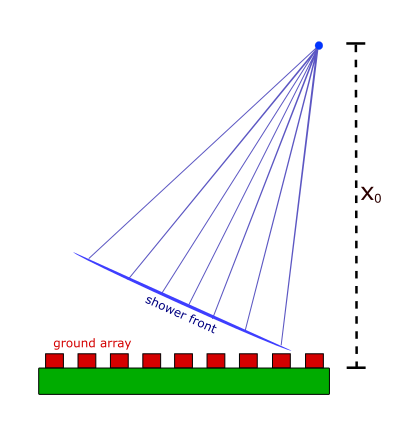
\includegraphics[width=\textwidth]{figures/airshower.png}
            \label{fig:my_label}
        \end{figure}
        
    
    \end{columns}
\end{frame}
%---------------------------------------------------------


%---------------------------------------------------------
\begin{frame}{Dataset, first glance}

    \begin{columns}
    
    \column{0.5\textwidth}
    \textbf{Dataset}: $10^5$ simulated events:
    \vspace{5 pt}

    \begin{itemize}
        \item[\textbullet] $9 x 9$ grid of detectors
        \item[\textbullet] most intense at center 
        \item[\textbullet] 80 frames of time series ($40$ $\si{MHz}$ sampling rate)
        \item[\textbullet] 1 frame of times of first arrival 
    \end{itemize}
    \vspace{10 pt}

    Single record shape: $(80 + 1 , 81)$\\
    \vspace{15 pt}

    \texttt{pd4ml} package splits by default in $70\%$ train $30\%$ test
    
    
    \column{0.5\textwidth}
        \begin{figure}
            \centering
            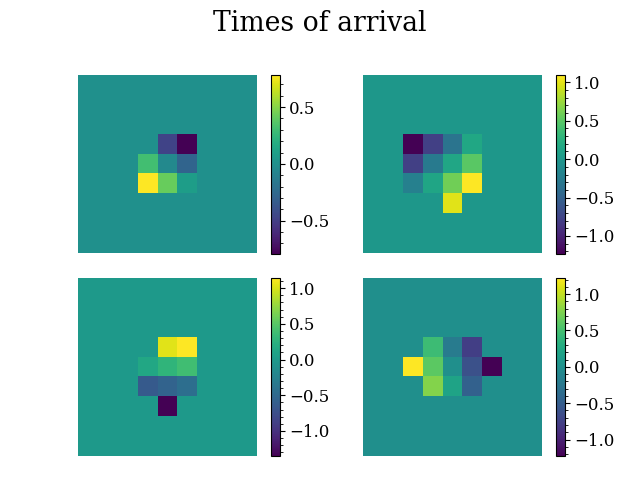
\includegraphics[width=0.8\textwidth]{figures/toa.png}
            \label{fig:my_label}
        \end{figure}
        
         \begin{figure}
            \centering
            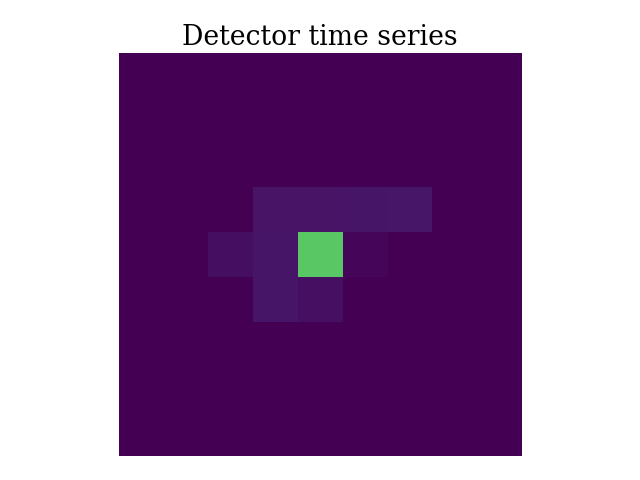
\includegraphics[width=0.65\textwidth]{figures/ezgif.com-gif-maker.png}
            \label{fig:my_label}
        \end{figure}
    
    \end{columns}

\end{frame}

%---------------------------------------------------------

\section{Preprocessing}

%---------------------------------------------------------
\begin{frame}{Split the dataset}

    \begin{columns}
    
    \column{0.6\textwidth}
    Dataset was already split in test and train.\\
    \vspace{10 pt}
    We put it all back together, shuffled it and divided with the following percentage:
    \begin{itemize}
        \item[\textbullet] $70\%$ \textit{train}
        \item[\textbullet] $20\%$ \textit{test}
        \item[\textbullet] $10\%$ \textit{validation}
        
    \end{itemize}
    \vspace{10 pt}

    For the design of the net it is convenient using \texttt{numpy} structured arrays
    
    
    \column{0.4\textwidth}
    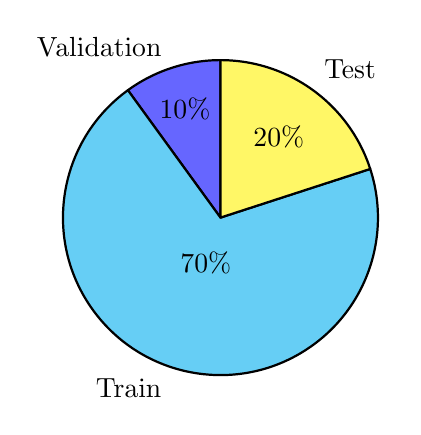
\begin{tikzpicture} %PIE CHART
    \pie[radius=2, rotate=90]{
    10/Validation,
    70/Train,
    20/Test}
    \end{tikzpicture}
    
    
    \end{columns}

    

\end{frame}

%---------------------------------------------------------
\begin{frame}[fragile]{Split the dataset: \texttt{funky\_dtype}}

    
    \begin{lstlisting}[language=Python]
    # custom numpy dtype
    funky_dtype = np.dtype(
        [
            ("outcome", np.float64),
            ("time_series", np.float32, (80, 81)),
            ("toa", np.float32, (9, 9, 1)),
        ])
    \end{lstlisting}
    
    All data relative to a single event is clustered in a single \texttt{numpy} object, transformation is:
    
    %Data is extracted: from a conceptually \emph{ihomogeneous} list 
    %(activity time series together with times of arrival) to
    \begin{equation*}
        (80 + 1, 81)\,\,\, \longrightarrow \,\,\, [("toa", (9, 9, 1)), ("timeseries", (80, 9,9))]
    \end{equation*}
    Data can be accessed "as a dictionary", depending on what is needed.

\end{frame}


%---------------------------------------------------------
\begin{frame}{\texttt{DataFeeder} class}
    Ensures an easy way to train the subnets separately %MA CHE VUOL DIRE?
    Class \texttt{DataFeeder} main features:
    \begin{itemize}
        \item[\textbullet] shuffles data randomly
        \item[\textbullet] input fields can be specified
        \item[\textbullet] can be extended to more complex training strategies
        \item[\textbullet] returns a generator
    \end{itemize}
    
    % QUESTO SI DICE A VOCE
    %The effect of the high reading time from memory ($\approx 3 m$s) is mitigated
    %by \texttt{keras} multiprocessing

\vspace{20 pt}
    %questa è la parte che c'era in "split the dataset", non c'entra con quello
    Using a generator (\texttt{keras.utils.Sequence})
    \begin{itemize}
        \item[\textbullet] inherit multiprocessing features
        \item[\textbullet] has default callbacks
        \item[\textbullet] avoids memory overload
    \end{itemize}
    
\end{frame}

%---------------------------------------------------------
\begin{frame}{\texttt{FeederProf(DataFeeder)} class}{Curriculum learning}
    
    Using a pre-trained network data can be ``scored'' and then sorted in ascending order of difficulty

    (work in progress) This can lead to a learning speed-up and improvements in resolution
    
    Caveat: this training strategy is not well suited (conceptually at least) for regression tasks, 
    since it is not clear what a ``difficult'' sample would look like.
\end{frame}

%---------------------------------------------------------
\begin{frame}{Data Augmentation}
%FORSE STA SLIDE LA SPOSETEREI DOPO
    Dataset has a lack of high events ($X > 850\si{m}$) so a first network training showed a worse resolution
    for samples corresponding to this range

    \begin{block}{Strategy}
        Increase the number of samples that overcome a certain heigth threshold using the
        symmetries of the problem
    \end{block}

    \begin{columns}
    \column{0.35\textwidth}
        Data is augmented using
    \begin{itemize}
        \item flip up-down
        \item flip left-right
        \item diagonal flip
        \item rotation of $90^{\circ}$
    \end{itemize}
    \column{0.65\textwidth}
    \begin{figure}
        \centering
        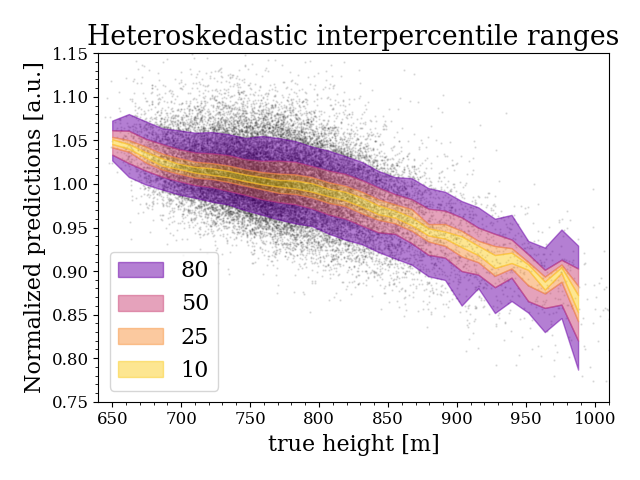
\includegraphics[width=0.7\textwidth]{figures/hetero1.png}
    \end{figure}
    \end{columns}
    
    %CI METTEREI UN GRAFICHELLO DELLA DISTRIBUZIONE DEI DATI IN ALTEZZA
    
    %only a subset of the available data undergoes this procedure.

    %Augmenting the whole dataset would leave the sample distribution unchanged and thus would not lead 
    %to improvements.
\end{frame}

\begin{frame}{Resolution}

    The reference article suggests using the resolution:
    \begin{block}{Resolution}
        defined as the standard deviation of the distribution given by the difference between the predictions and the actual values of $X_{max}$
    \end{block}

    We point out that 
    \[\sigma^2 = \frac{1}{N}\sum_i (\delta_i - \bar{\delta})^2\]
    is a sensible estimator of ``how much the net has gone wrong'' only if $\bar{\delta} = 0$, for which the adopted resolution is equal 
    to the $RMSE$ of the distribution
    \[ RMSE^2 = \frac{1}{N}\sum_i(x_i - \hat{x}_i)^2 \]
    Since (on a typical train) $\bar{\delta} \approx 10$m we preferred the RMSE.
\end{frame}



\section{Neural Network building}

    \centering
    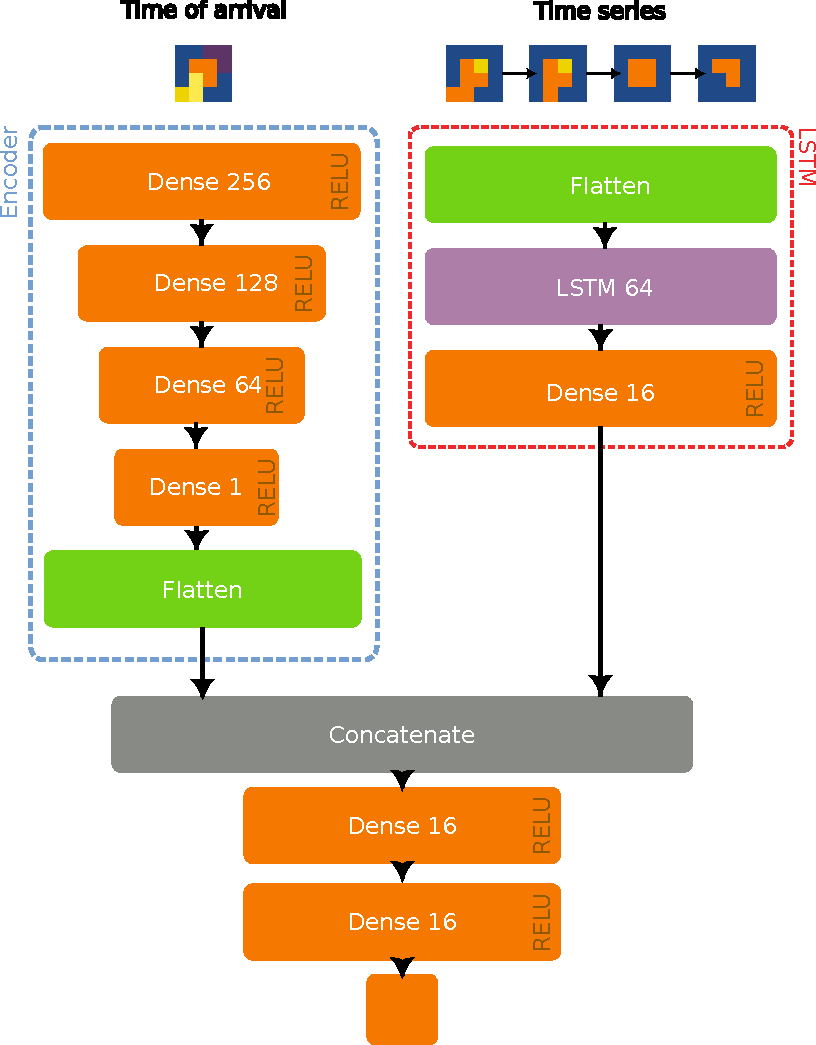
\includegraphics[width=0.6\textwidth]{figures/model.pdf}
%---------------------------------------------------------
\begin{frame}{Overview on the network}
    The assumption that lead to this design is that from the time of arrival matrix
    it is possible to infer some kind of ``homogeneous'' shower parameters (incidence angle, spread, etc.)
    while the time series can be processed by a recurrent network.
\end{frame}

%---------------------------------------------------------
\begin{frame}{Encoder for time of arrivals}

    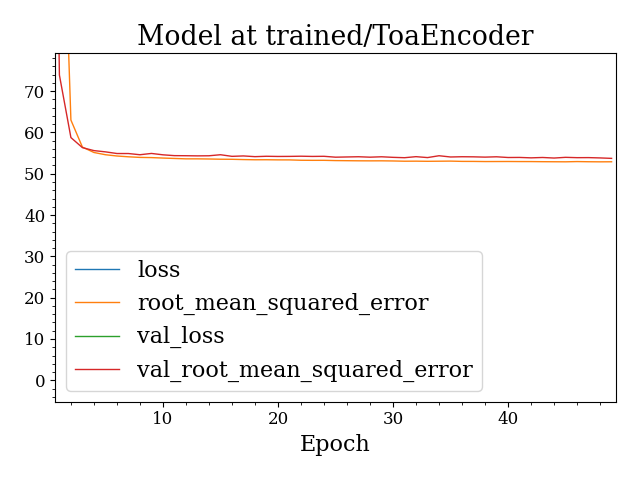
\includegraphics[width=\textwidth]{figures/ENC_history.png}
    
\end{frame}


%---------------------------------------------------------
\begin{frame}{LSTM}
    LSTM (\textit{Long Short Term Memory}) cell is a variant of a typical recurrent RNN cell.
    It is able to learn long-term dependencies that brings along in a hidden state.

    \begin{figure}
        \centering
        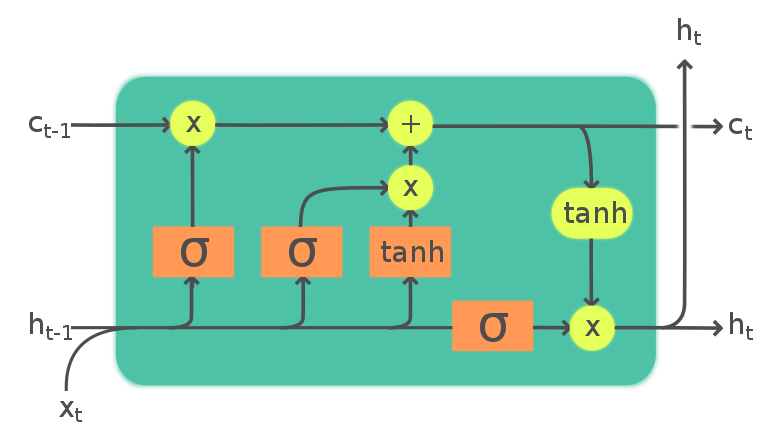
\includegraphics[width=0.7\textwidth]{figures/LSTM_Cell.svg.png}
        %\caption{Credits: Guillaume Chevalier}
    \end{figure}
    
    %maybe inserire grafici della sigma e del tanh
\end{frame}

%---------------------------------------------------------
\begin{frame}{LSTM for the time series}
    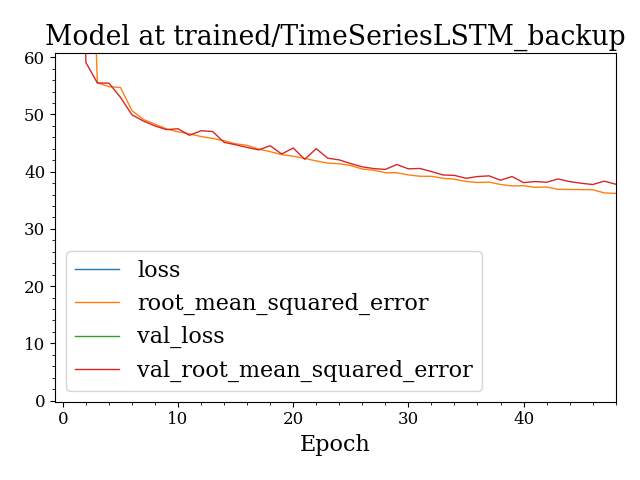
\includegraphics[width=\textwidth]{figures/LSTM_history.png}    
\end{frame}

\begin{frame}{Subnets performance}
    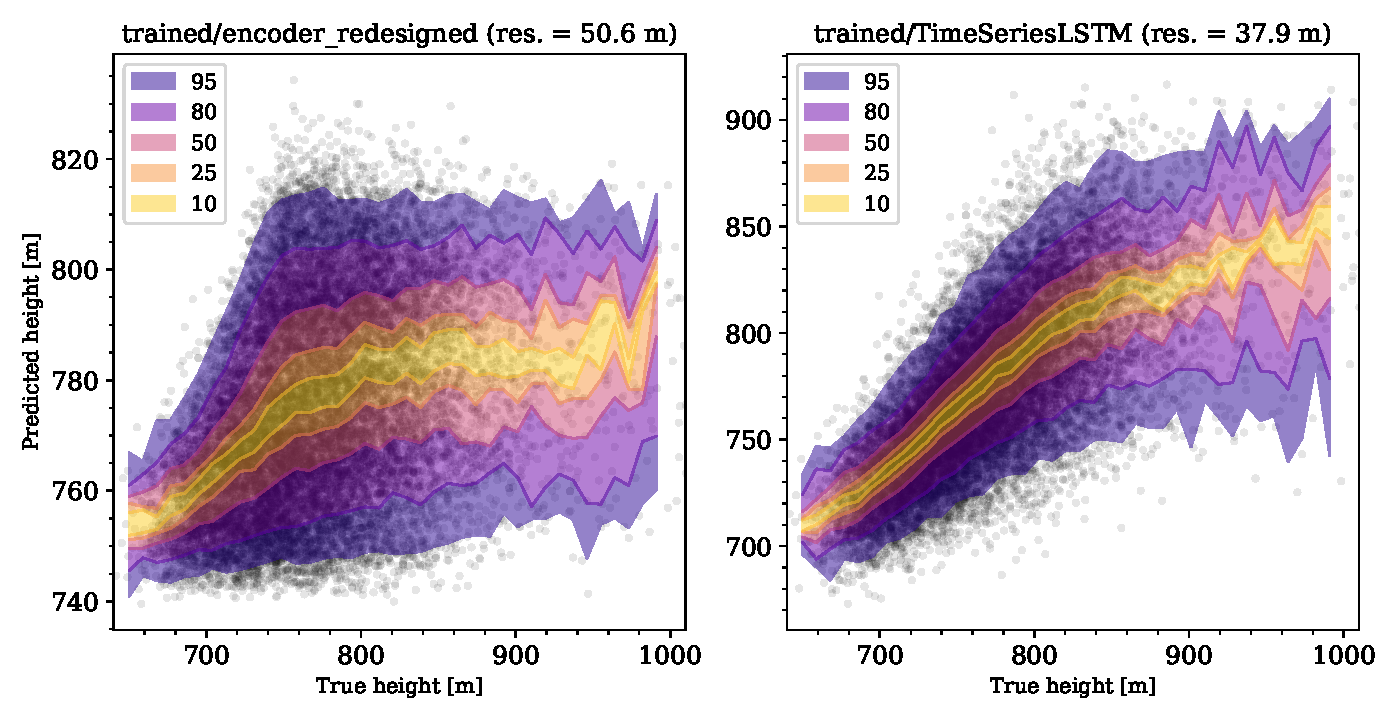
\includegraphics[width=\textwidth]{figures/sub_net_train.pdf}
\end{frame}

%---------------------------------------------------------
\begin{frame}{Concatente + dense layers}

    
\end{frame}


\begin{frame}{Subnets train freezing}
    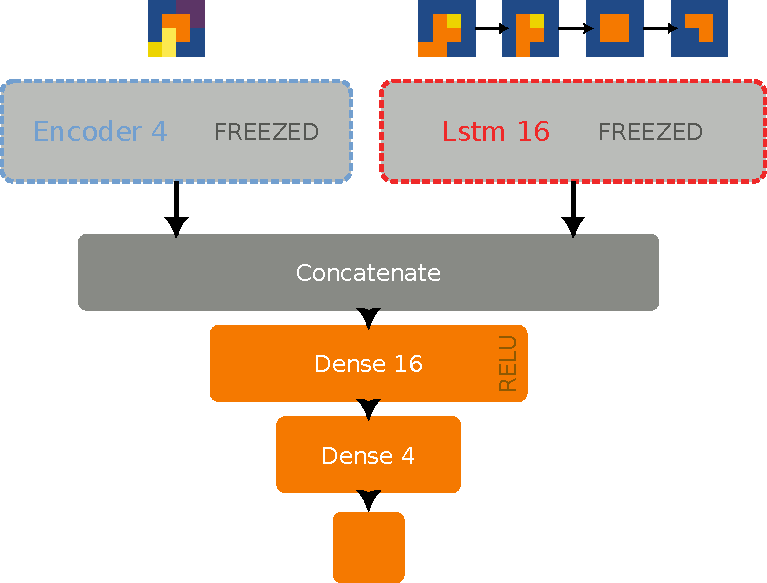
\includegraphics[width=.8\linewidth]{figures/freezetraining_2.pdf}
\end{frame}

\begin{frame}{Subnets train freezing}
    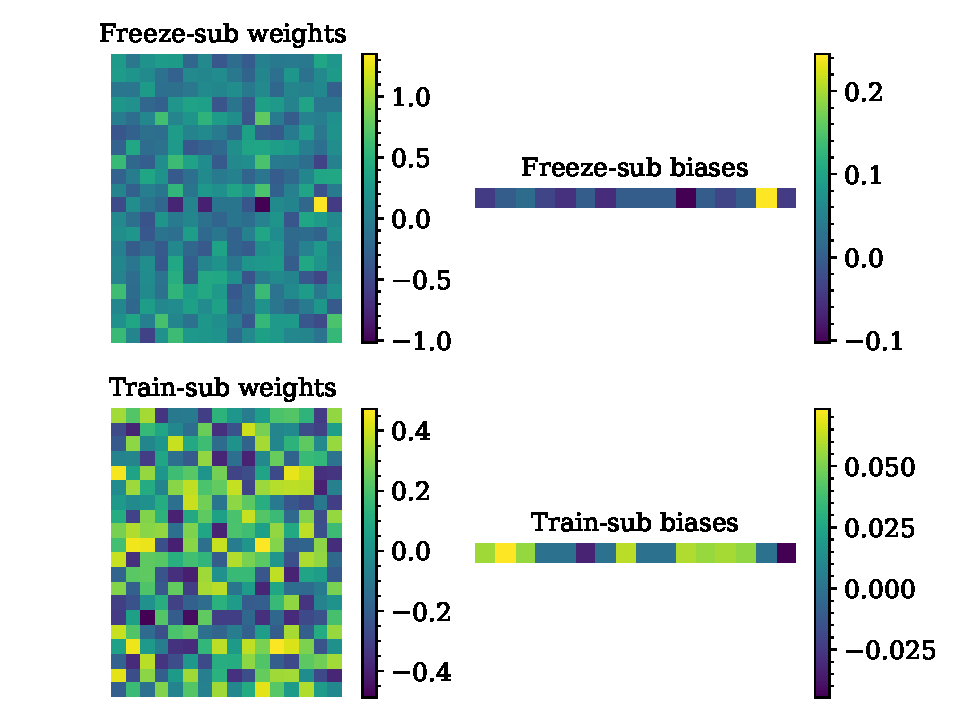
\includegraphics[width=.8\linewidth]{figures/freezetraining.pdf}
\end{frame}

%---------------------------------------------------------
\begin{frame}[fragile]{Network's output}
    \begin{lstlisting}[language=Python]
    import numpy as np
        
    def incmatrix(genl1,genl2):
        m = len(genl1)
        n = len(genl2)
        M = None #to become the incidence matrix
        string = "ciao"
      
    \end{lstlisting}

    
\end{frame}

%---------------------------------------------------------
\begin{frame}{Hyperparameters tuning}

    
\end{frame}


%---------------------------------------------------------
\begin{frame}{Whole Network performance}

    
\end{frame}

\begin{frame}{Test setup on CircleCI}

    
\end{frame}

%---------------------------------------------------------
\begin{frame}{Danke e bibliography}
\centering
Danke Schon

    
\end{frame}




\end{document}